\section{Numerical experiments}\label{sec:numerics}
Having constructed strong stability preserving $TM^{n-2}R$ schemes in the previous
section, we now numerically verify their properties.
%where $M$ is an ESSPRK($s,q,p$) scheme and
%$R$ and $T$ are its associated SSP starting and stopping schemes from
%Section~\ref{subsec:starting_stopping}.
Specifically, we use a convergence study to show that the procedure
attains order of accuracy $q$, the effective order of $M$.
We also demonstrate on Burgers' equation that the
SSP coefficient accurately measures the maximal time-step for which the
methods are strong stability preserving.

\subsection{Convergence study}\label{subsec:convergence}
We consider the van der Pol system \cite{Hairer1987_book}
\begin{equation}\label{eq:conv_eq}
	\begin{split}
    		u_1'(t) &= u_2(t), \\
                u_2'(t) &= \mu \bigl(1 - u_1^2(t)\bigr)u_2(t) - u_1(t),
    \end{split}
\end{equation}
over the time interval $t \in [0, 50]$ with $\mu = 2$ and initial
values $u_1(0) = 2$ and $u_2(0) = 1$.
The reference solution for the convergence study is calculated by \textsc{Matlab}'s 
\texttt{ode45} solver with relative and absolute tolerances set to $10^{-13}$.

We solve the initial value problem \eqref{eq:conv_eq}
using SSP $TM^{n-2}R$ schemes.
% where $M$ is effective order three and four and classical order two.
The solution is computed using $n = 100 \cdot 2^{k}$ time steps for
$k = 2, \dots, 7$.
The error at $t = 50$ with respect to time-step is shown in 
Figure~\ref{fig:conv_study} on a logarithmic scale.
\begin{figure}
	\centering
     \subfloat[ESSPRK($s,3,2$)]{\label{fig:conv_study_a}
     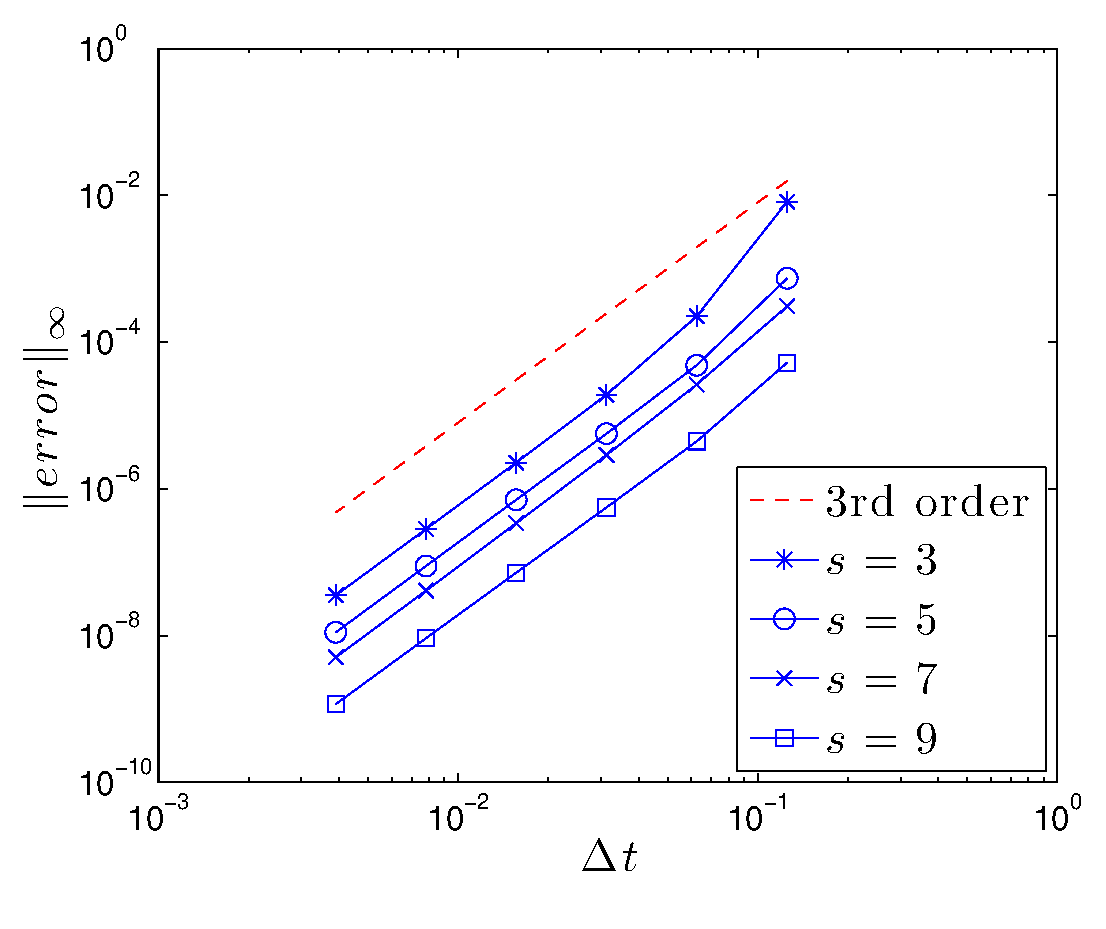
\includegraphics[width=0.48\textwidth]{Pictures/convergence_3_order}}
   \quad
     \subfloat[ESSPRK($s,4,2$)]{\label{fig:conv_study_b}
    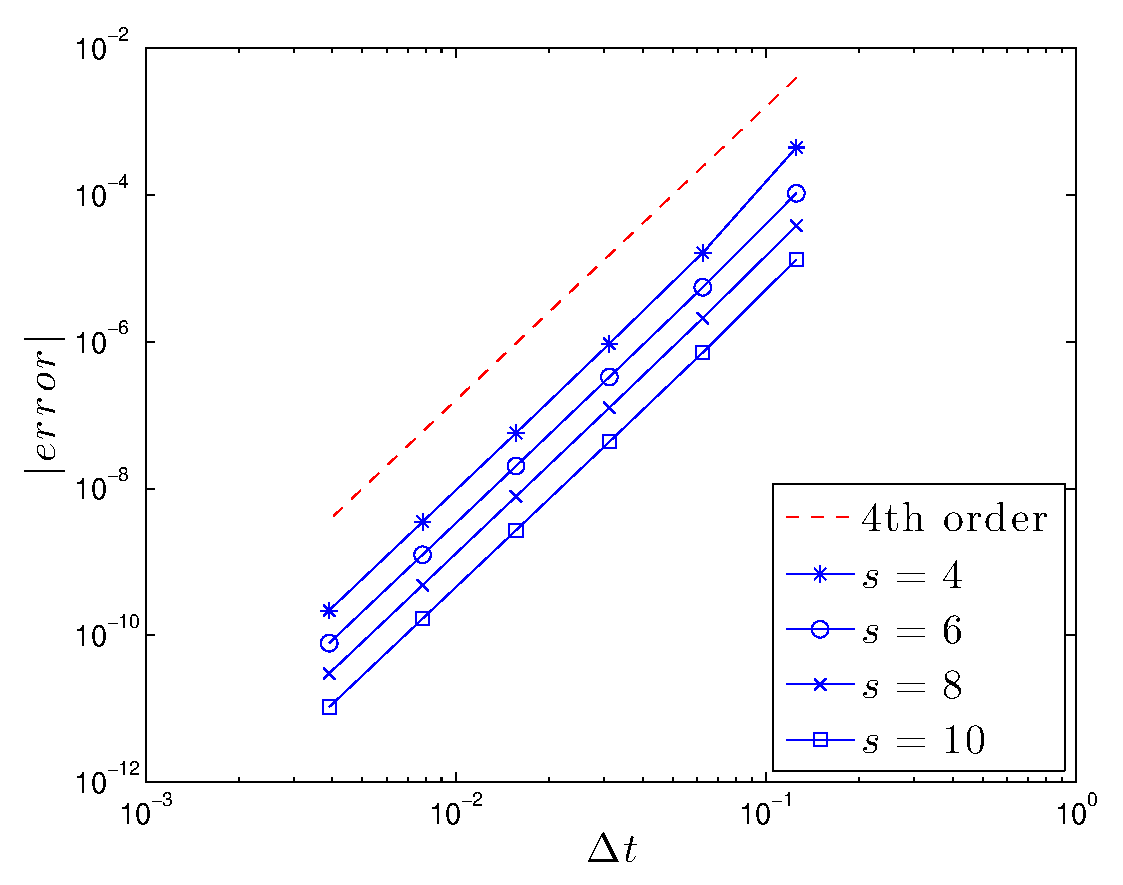
\includegraphics[width=0.48\textwidth]{Pictures/convergence_4_order}}
    \caption{Convergence study of $TM^{n-2}R$ Runge--Kutta schemes when (a) $M$
    is an ESSPRK($s,3,2$) method and (b) $ M $ is an ESSPRK($s,4,2$) method.}
    \label{fig:conv_study}
\end{figure}
The convergence study is performed for $TM^{n-2}R$ schemes with
various number of stages $s$ and the results show that the schemes
attain an order of accuracy equal to the effective order of their main
method $M$.
It is important in doing this sort of convergence study that the
effective order of accuracy can only be obtained after the stopping method is
applied.
Intermediate steps will typically only be order $p$ accurate (the classical
order of the main method).
Finally, we note that the methods with more stages generally exhibit smaller errors
(for a given step size).

\subsection{Burgers' equation}\label{subsubsec:burgers}
The inviscid Burgers' equation consists of the scalar hyperbolic conservation law
\begin{align}\label{eq:HCL}
    U_{t} + f(U)_{x} = 0,
\end{align}
with flux function $f(U) = \frac{1}{2}U^{2}$. 
We consider initial data
$U(0,x)  = \frac{1}{2} - \frac{1}{4}\sin{\pi x}$,
on a periodic domain $x \in [0,2)$.
The solution advances to the right where it eventually exhibits a shock. 
We perform a semi-discretization
using an upwind approximation to obtain the system of ODEs
\begin{align*}\label{eq:burgers_flux}
	\frac{\textrm{d}}{\textrm{d} t} u_i = -\frac{f(u_{i}) - f(u_{i-1})}{\Delta x}.
\end{align*}
This spatial discretization is total-variation-diminishing (TVD) when
coupled with the forward Euler method under the restriction
\cite{Laney:1998}  %,Ketcheson/Macdonald/Gottlieb:2009}.
$$\Dt \leq {\Dt}_{\text{FE}} = \Delta x / \|U(0,x)\|_{\infty}.$$
Recall that a time discretization with SSP
coefficient $\sspcoef$ will give a TVD solution for $\Dt \leq
\sspcoef {\Dt}_{\text{FE}}$.

Burgers' equation was solved using an SSP $TM^{n-2}R$ scheme with time-step
restriction $\Dt \leq \sigma{\Dt}_{\text{FE}}$, where $\sigma$ indicates the size 
of the time step. 
We integrate to roughly time $t_\text{f} = 1.62$ with $200$ points in space.
Figure~\ref{fig:burgers_cont} shows that if $\sigma$ is chosen less than the SSP
coefficient of the main method, then no oscillations are observed. 
If this stability limit is violated, then oscillations may appear.

We measure these oscillations by computing the total variation of the 
numerical solution.
When $M$ is an ESSPRK($4,4,2$) method,
it turns out that $\sigma = 1.57$ is the largest value of $\sigma$
for which the total variation is monotonically decreasing during the
calculation.
This is $79\%$ larger than the value of the SSP coefficient $\sspcoef = 0.88$.

\begin{figure}
    \centering
    \subfloat[$\sigma = 0.88$]{\label{fig:burgers_cont_a}
      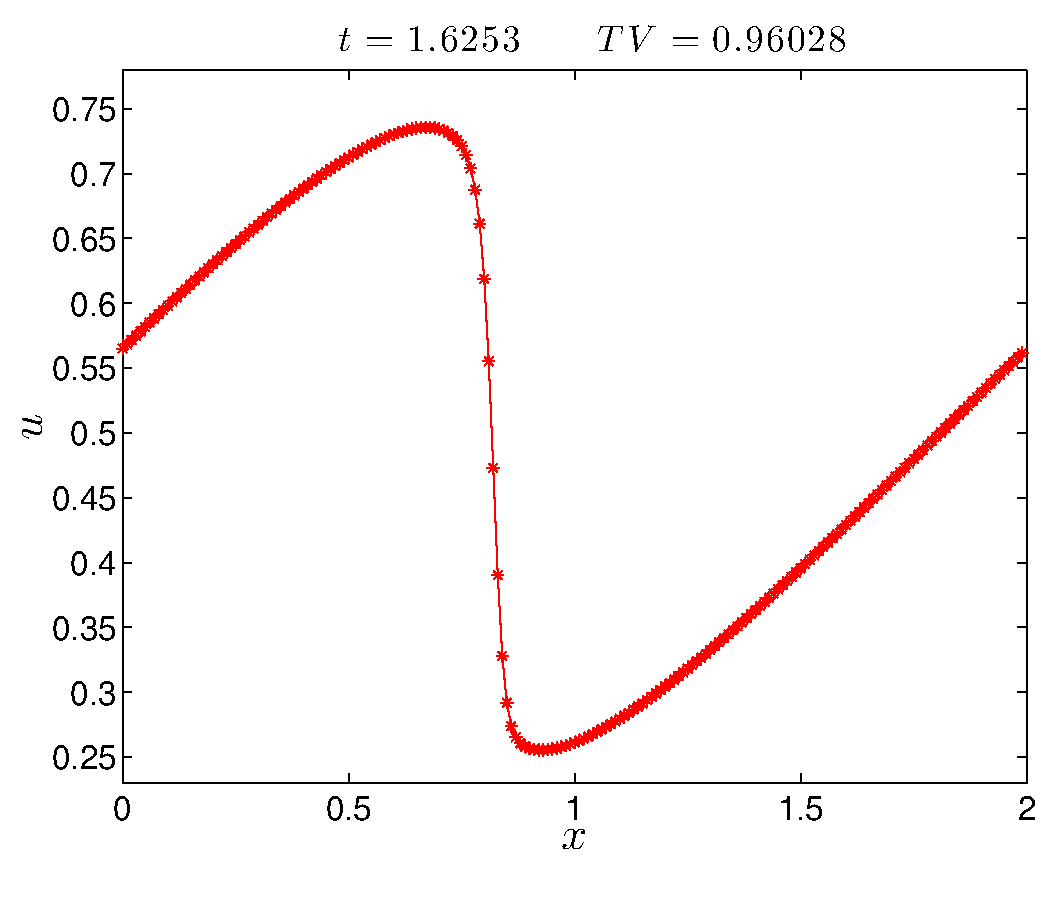
\includegraphics[width=0.48\textwidth]{Pictures/burgers_cont}}\;
    \subfloat[$\sigma = 1.60$]{\label{fig:burgers_cont_b}
      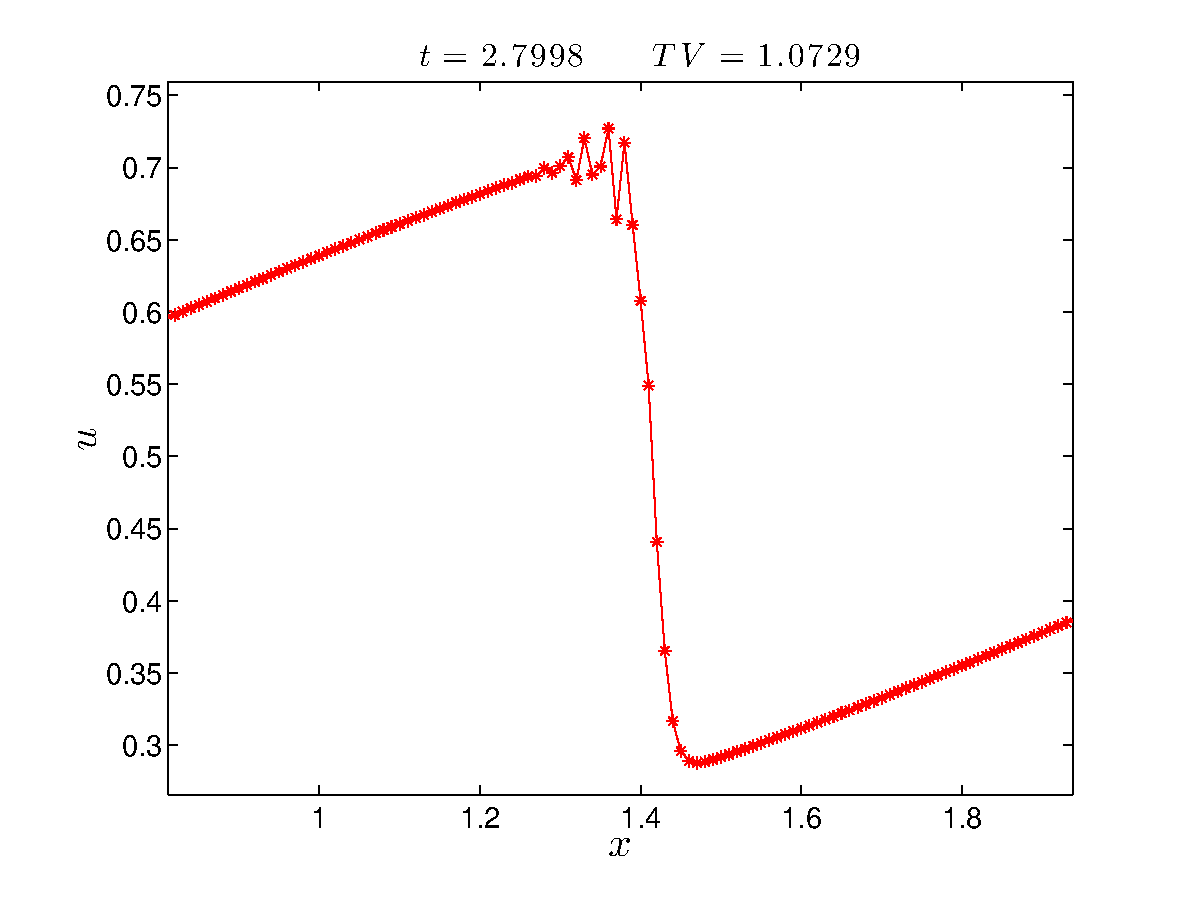
\includegraphics[width=0.48\textwidth]{Pictures/burgers_cont_no_tvd}}
    \caption{Solution of Burgers' equation at the final time with continuous initial data, using a
    $TM^{n-2}R$ scheme, where $M$ is the optimal ESSPRK($4,4,2$). 
    The SSP coefficient is $\sspcoef = 0.88$. 
    Figure~\ref{fig:burgers_cont_b} shows a zoom in the region of space where
    oscillations appear.
    Here $TV$ denotes the $TV$-norm of the solution at the final time:
    a value greater than 1 (the $TV$-norm of the initial condition)
    indicates a violation of the TVD condition.
    %Note that the solution in Figure~\ref{fig:burgers_cont_b} is
    %monotonically increasing at intermediate steps as well.
    }
    \label{fig:burgers_cont}
\end{figure}

We also consider Burgers' equation with a discontinuous
square wave initial condition
\begin{equation}\label{eq:burgers_discont_IC}
    U(0,x)  = \left\{
                \begin{array}{ll}
                  1, & \hbox{$0.5 \leq x \leq 1.5$} \\
                  0, & \hbox{otherwise.}
                \end{array}
              \right.
\end{equation}
The solution consists of a rarefaction (i.e., an expansion fan) and a
moving shock.
Again we use $200$ points in space and we compute the solution until
roughly time $t_\text{f} = 0.6$.
Figure~\ref{fig:burgers_discont} shows the result of solving the
discontinuous problem using an SSP $TM^{n-2}R$ scheme, where $M$ is an
ESSPRK($5,4,2$) method with SSP coefficient $\sspcoef = 1.95$.
In this case, $\sigma = 1.98$ appears to be the largest value
for which the total variation is monotonically decreasing during the 
calculation.
This is $2\%$ larger than the value of the SSP coefficient.
Figure~\ref{fig:burgers_discont_b} shows part of the solution exhibiting 
oscillations when $\sigma$ is larger than the SSP coefficient.
For various schemes, Table~\ref{tab:observed_SSP_coeff} shows the
maximum observed values of $\sigma$ for which the numerical solution
is total variation decreasing for the entire computation.
With the exception of the four-stage effective order four methods, we
note good agreement between the SSP coefficient predicted by the
theory and the maximum time-step for which the numerical solution is
TVD.

\begin{figure}
    \centering
    \subfloat[$\sigma = 1.95$]{\label{fig:burgers_discont_a}
      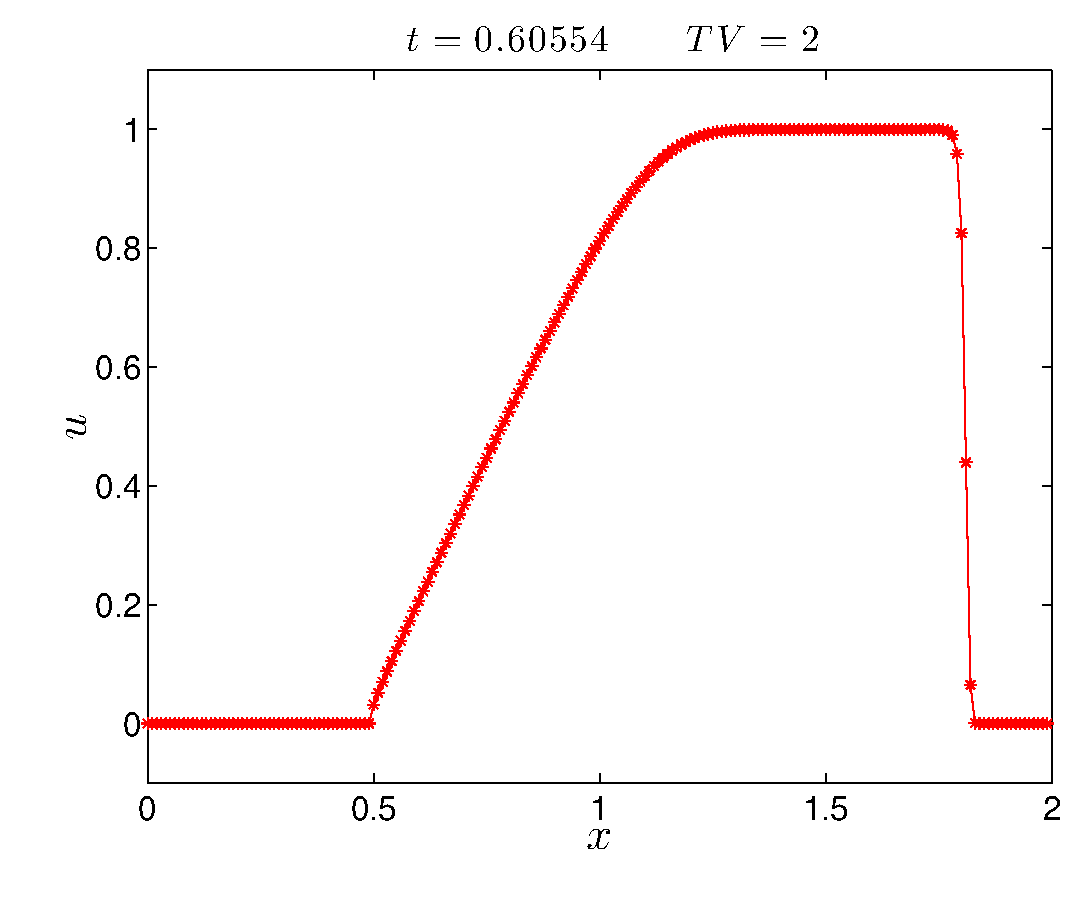
\includegraphics[width=0.48\textwidth]{Pictures/burgers_discont}}\;
    \subfloat[$\sigma = 2.15$]{\label{fig:burgers_discont_b}
      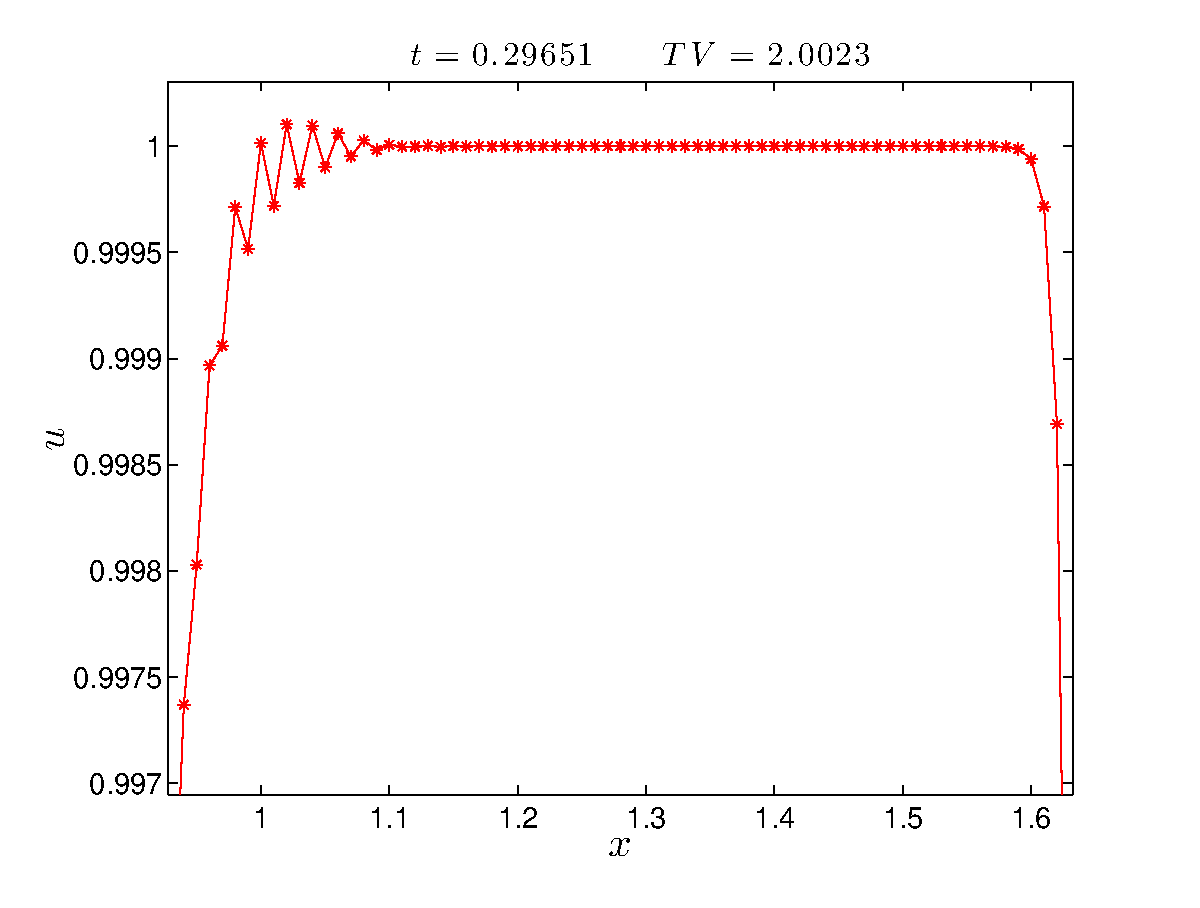
\includegraphics[width=0.48\textwidth]{Pictures/burgers_discont_no_tvd}}
    \caption{Solution of Burgers' equation at the final time with discontinuous initial data, using a
    $TM^{n-2}R$ scheme, where $M$ is ESSPRK($5,4,2$) method. 
    The SSP coefficient is $ \sspcoef = 1.95$.
    Figure~\ref{fig:burgers_discont_b} shows a zoom in the region of space where
    oscillations appear.
    Here $TV$ denotes the $TV$-norm of the solution at the final time:
    a value greater than 2 indicates a violation of the TVD condition.
    %Note that the solution in Figure~\ref{fig:burgers_discont_b} is
    %monotonically increasing at intermediate steps as well.
    }
    \label{fig:burgers_discont}
\end{figure}

\begin{table}
    \centering
    \begin{tabular}{ccc@{\hspace{5pt}} c@{\hspace{5pt}} c@{\hspace{5pt}} c@{\hspace{5pt}} c@{\hspace{5pt}} c@{\hspace{5pt}} c@{\hspace{5pt}} c@{\hspace{5pt}} c@{\hspace{5pt}}}
        \hline
        %\multicolumn{2}{|c|}{\backslashbox{\hspace{2pt}\vspace{1pt}$q\,,\,p$}{\vspace{-5.5pt}$s$}} & $3$ & $4$ & $5$ & $6$ & $7$ & $8$ & $9$ & $10$ & $11$ \\
        \multirow{2}{*}{$q$} &
        \multirow{2}{*}{\;\;$p$\;\;}
               &   \multicolumn{9}{c}{stages $s$} \\
            \cline{3-11}
        &      &   $3$ & $4$ & $5$ & $6$ & $7$ & $8$ & $9$ & $10$ & $11$ \\
        \hline
        $3$ & $2$ & \small$1.04(4\%)$ & \small$2.00(0\%)$ & \small$2.65(0\%)$ & \small$3.52(0\%)$ & \small$4.29 (0\%)$ & \small$5.11(0\%)$ & \small$6.00(0\%)$ & \small$6.79(0\%)$ & \small$7.63(0\%)$\\
        $4$ & $2$ & \small$-$ & \small$1.07(22\%)$ & \small$1.98(2\%)$ & \small$2.69(2\%)$ & \small$3.56(1\%)$ & \small$4.33(1\%)$ & \small$5.16(1\%)$ & \small$6.05(1\%)$ & \small$6.84(1\%)$ \\
        $4$ & $3$ & \small$-$ & \small$1.05(35\%)$ & \small$1.89(3\%)$ & \small$2.63(2\%)$ & \small$3.53(1\%)$ & \small$4.31(1\%)$ & \small$5.16(1\%)$ & \small$6.04(1\%)$ & \small$6.85(1\%)$ \\
    \end{tabular}
    \caption{Maximum observed coefficients exhibiting the TVD property on 
    the Burgers' equation example with discontinuous data \eqref{eq:burgers_discont_IC}.
    The numbers in parenthesis indicate the increase relative to the corresponding SSP
    coefficients.}
    \label{tab:observed_SSP_coeff}
\end{table}
    
We also note the necessity of our modified starting and stopping methods in the $RM^{n-2}T$ approach: in this
example if we use the original approach of $S$ and $S^{-1}$,
the solution exhibits oscillations immediately following the
application of the starting perturbation method $S$.
%This is illustrated in Figure~\ref{fig:burgers_starting_method}
%\yiannistodo{Shall we include a plot about this?}
%Colin: fine as is for now


%It is interesting to note that the stability prediction of the SSP
%coefficient for ESSPRK is quite tight compared to other SSP methods
%(c.f., \cite[Table 5.1]{Ketcheson/Gottlieb/Macdonald:TSRK}).
%Moreover it becomes sharper as the number of spatial points increases,
%since the dissipation of the numerical solution is decreased.
%This may make effective order methods an interesting test case for
%further research into both SSP time-discretizations as well as spatial
%discretizations with strong stability features.
% TODO: we probably want a table here to support this...



% The ESSPRK-scheme preserves monotonicity in the TV-norm since the starting 
% method $R$ is SSP.
% Using the original approach with $S$ and $S^{-1}$, the results are not
% SSP and the total-variation increases after the perturbation $S$.
% This is illustrated in Figure~\ref{fig:burgers_starting_method} in which 
% the solution is plotted after one application of methods $R$ and $S$ as the 
% starting procedures.
% % Note: its not really a step for %S% so I said application
% \begin{figure}
%     \centering
% 	TODO
% 	\yianniscomment{This should be cut out since if we optimize directly for R and T, we are not mentioning S.}
%     \caption{Solution of Burgers' equation with discontinuous initial data 
%     after one step, using a $TM^{n-2}R$ scheme, where $M$ is an 
%     SSPRK($5,4,2$) method. The solution is advanced one step by using (a) $R$ and 
%     (b) $S$}
%     \label{fig:burgers_starting_method}
% \end{figure}

